\documentclass[a4paper,10pt,landscape,twocolumn]{scrartcl}

%% Settings
\newcommand\problemset{3}
\newcommand\deadline{Wednesday September 19th, 21:00h}
\newif\ifcomments
\commentsfalse % hide comments
%\commentstrue % show comments

% Packages
\usepackage[english]{{../exercises}}
\usepackage{wasysym,hyperref,graphicx}

\begin{document}

\practiceproblems

{\sffamily\noindent
This week's exercises deal with discrete random variables. You do not have to hand these exercises in; they are optional and for practicing only. If you have questions about them, please post them to the \href{https://www.moodle.ch/lms/mod/forum/view.php?id=1634}{discussion forum} and try to help each other. We will also keep an eye on that.
}
%%%%%%%%%%%%%%%%%%%%%%%%%%%%%%%%%%%%%%%%%%%%%%%%%%%%%%%%%%%%


\begin{exercise}[]
Let $X$ be a random variable taking any of the values $0, 5, -5$ with probabilities $P(X=-5) = P(X	= 0) = 0.3$ and $P(X=5) = 0.4$. What is $E[X^2]$?
\end{exercise}

\begin{exercise}[]
Compute the pmf of the number of tails for 7 subsequent coin tosses.	
\end{exercise}

\begin{exercise}[]
	Calculate the variance of a loaded 6-sided die that has a probability of $\frac 1 6$ for all odd numbered sides and $P(\{2\}) = P(\{4\}) =0.1$ and $P(\{6\}) = 0.3$.
\end{exercise}

%\begin{exercise}[]
%	You are betting with a friend. If Ajax wins this year's national football competition, your friend has to pay you $C$ euros. If you estimate Ajax to win with probability $p$ in this one-year period, what should you charge him
%\end{exercise}

\begin{exercise}[Independence]
Three events $A$, $B$, and $C$ are pairwise independent if each pair is independent. They are mutually independent if they are pairwise independent and in addition
	\begin{align}\label{eq:pairwise-indep}
		P(A \cap B \cap C) = P(A) P(B) P(C) \, .
	\end{align}
	\begin{subex}
	Suppose we roll two 6-sided dice. Consider the events:
	\[
		D = \text{`odd on die 1'} \quad
		E = \text{`odd on die 2'} \quad
		F = \text{`odd sum'}
	\]
	Are $D$, $E$, and $F$ pairwise independent? Are they mutually independent?	
	\end{subex}
	
	\begin{subex}
		Consider the Venn diagram in figure \ref{fig:venn}. $A$, $B$ and $C$ are the overlapping circles and the probabilities of each region are as marked. Does equation \ref{eq:pairwise-indep} hold? Are the events $A$, $B$, $C$ mutually independent?
	\end{subex}
	
	\begin{subex}
	For families with $n$ children, the events ``the family has children of both sexes'' and ``there is at most one girl'' are independent. What is $n$?
	\end{subex}


\end{exercise}

\begin{figure}\centering
	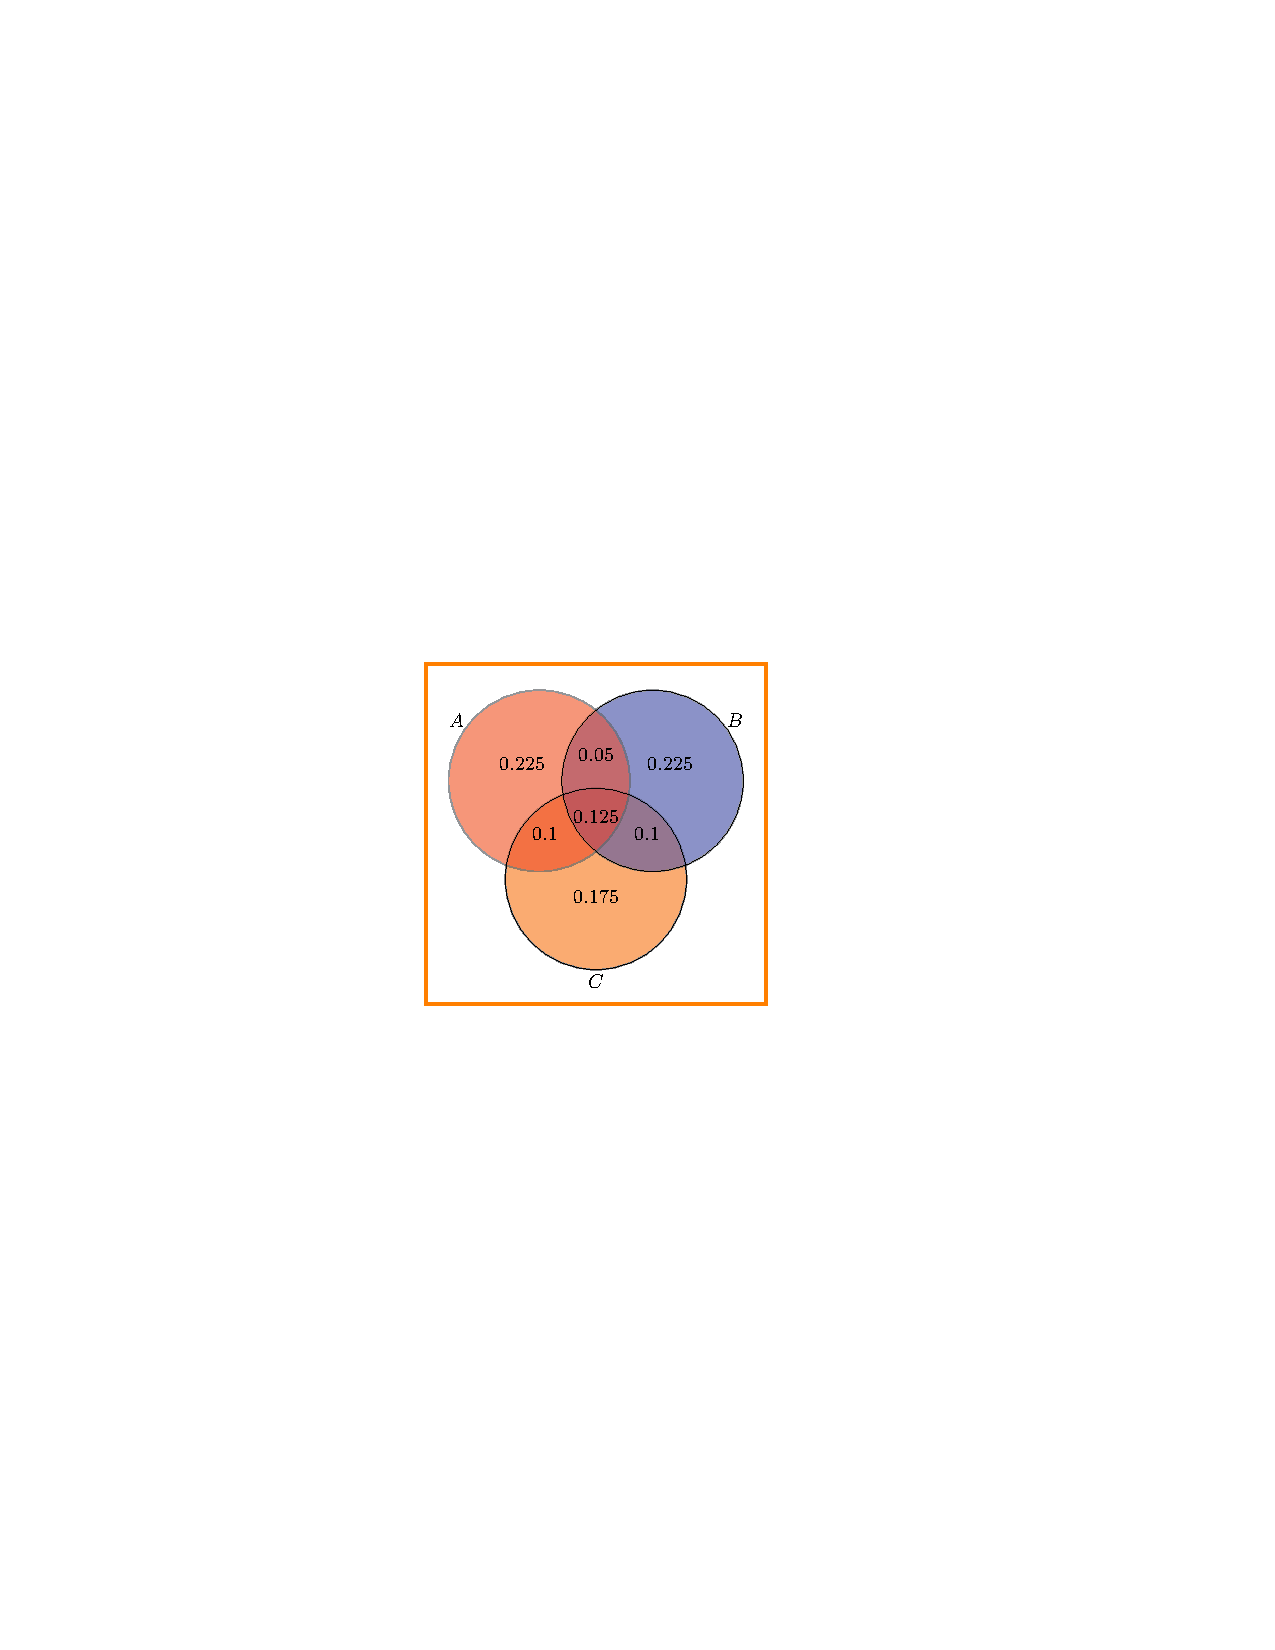
\includegraphics[width=.2\textwidth]{03-venn}	
	\caption{Venn diagram for problem 4 (b)\label{fig:venn}}
\end{figure}



\begin{exercise}[Trees of cards]
There are $8$ cards in a hat:
	\[
		\{1\heartsuit, 1\spadesuit, 1\diamondsuit, 1\clubsuit, 2\heartsuit, 2\spadesuit, 2\diamondsuit, 2\clubsuit\}.
	\]
You draw one card at random. If its rank is 1 you draw one more card;
if its rank is two you draw two more cards. Let $X$ be the sum of the
ranks on all the cards you have drawn. Find $E(X)$.
	
\end{exercise}

\begin{exercise}[Seating arrangements]
	A total of $n$ people take their seats around a circular table with $n$ chairs. No two people have the same height. What is the expected number of people who are shorter than both of their immediate neighbours?
\end{exercise}


%\begin{exercise}
%Boxes of cereal are 30cm tall. Due to settling, boxes have a higher density of raisins at the bottom ($h=0$) than at the top ($h=30$). Suppose the density (in raisins per cm of height) is given by $f(h) = 40-h$.
%	\begin{subex}
%	How many raisins are in a box?	
%	\end{subex}
%	\begin{subex}
%		Let $H$ be the height of a random raisin
%	\end{subex}
%	
%\end{exercise}


\begin{exercise}[Negative binomial distribution]
 Assume that a number of independent trials, each with a probability of success of $p$, $0 < p < 1$, are performed until $q$ successes are registered. Let $X$ be equal to the number of trials required, then
	$$P(X = n) = {{n-1} \choose {q-1}} p^{q} (1 - p)^{n-q} \qquad \qquad n = q, q+1, ...$$

	Any RV $X$ whose probability distribution is given by the above is said to be a {\em negative binomial RV} with parameters $(q,p)$. Compute the expectation and variance of this RV with parameters $(q,p)$.	
\end{exercise}

\vfill
\credits{Some questions are from MIT course 18-05 by Jeremy Orloff and Jonathan Bloom, see ocw.mit.edu.}
\end{document}